\documentclass{article}
\usepackage[margin=1in]{geometry}
\usepackage{microtype}
\usepackage{setspace}
\usepackage{amsmath}
\usepackage{parskip}
\usepackage{amssymb}
\usepackage{graphicx}

\graphicspath{{../public/}}

\parskip=4ex
\date{}
\author{}

\title{12.2 Double Integrals Over General Regions}

\begin{document}
  \maketitle
  When integrating a function $ f $ over regions $ D $ that on a more general shape as opposed to rectangles, we suppouse that $ D $ is a bounded region. Meaning $ D $ can be enclosed in a rectangular region $ R $. A new function $ F $ with domain $ R $ can defined like so
  \[
    F(x,y) = 
    \begin{cases}
      f(x,y) \qquad \text{if $ (x,y) $ is in $ D $ }\\
      0 \qquad \text{if $ (x,y) $ is in $ R $ but not $ D $ }
    \end{cases}
  \]

  \begin{center}
    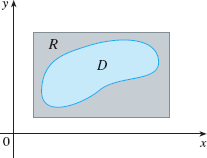
\includegraphics[width=6cm]{12_2_1}
  \end{center}

  If the double integral of $ F $ exists over $ R $, then the double integral of $ f $ over $ D $ is defined by
  \[
    \iint_D f(x,y)~dA = \iint_R F(x,y)~dA
  \]
 
  A plane region $ D $ is of type I if it lies between the graphs of two continuous functions of $ x $, that is
  \[
    D= \{ (x,y)| a \le x \le b, g_1(x) \le y \le g_2(x) \}
  \]

  Examples of type I plane regions
  \begin{center}
    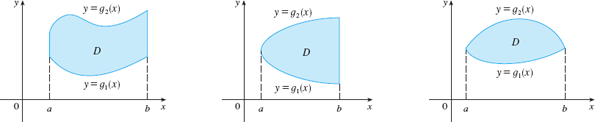
\includegraphics[width=6cm]{12_2_2}
  \end{center}

  In order to evaluate $ \iint_D f(x,y)~dA $ when $ D $ is a region of type I, we choose a rectangle $ R = [a,b] \times [c,d] $ that contains $ D $. Let $ F $ be the function
  \[
    F(x,y) = 
    \begin{cases}
      f(x,y) \qquad \text{if $ (x,y) $ is in $ D $ }\\
      0 \qquad \text{if $ (x,y) $ is in $ R $ but not $ D $ }
    \end{cases}
  \]

  Meaning $ F $ is 0 outside $ D $ or in a simpler context, $ F $ is $ 0 $ when $ y < g_1(x) $ or $ y > g_2(x) $. Then by Fubini's Theorem,
  \[
    \iint_D f(x,y)~dA = \iint_R F(x,y)~dA = \int^{b}_{a} \int^{d}_{c} F(x,y) ~dydx 
  \]

  If $ f $ is continuous on a type I region $ D $ such that
  \[
    D = \{ (x,y) | a \le x \le b, g_1(x) \le y \le g_2(x) \}
  \]
  then
  \[
    \iint_D f(x,y)~dA = \int^{b}_{a} \int^{g_2(x)}_{g_1(x)} f(x,y) ~dydx 
  \]

  Observe the right hand integral is an iterated integral, however within the inner integral, $ x $ is regarded as a constant not only in $ f(x,y) $, but also in the limits of integration, $ g_1(x) ~\&~ g_2(x) $.

  Consider plane regions of type II, which is expressed as
  \[
    D = \{ (x,y) | c \le y \le d, h_1(y) \le x \le h_2(y) \}
  \]

  Where $ h_1 ~\&~ h_2 $ are continuous. Consider some examples of type II plane regions below.
  \begin{center}
    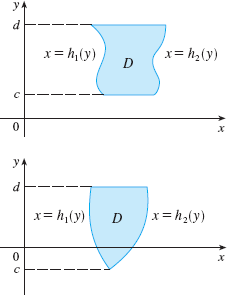
\includegraphics[width=6cm]{12_2_3}
  \end{center}
  
  Plane regions of type II can be integrated like below
  \[
    \iint_D f(x,y)~dA = \int^{d}_{c} \int^{h_2(x)}_{h_1(x)} f(x,y) ~dxdy
  \]
 
  Evaluate $ \iint_D (x+2y)~dA $ where $ D $ is the region bounded by the parabolas $ y=2x^{2} ~\&~ y=1+x^{2}$

  The parabolas intersect when $ 2x^{2}=1+x^{2} $ and by solving for x we get $ \pm1 $. $ D $ is also a type I region so we write
  \[
    D = \{ (x,y) | -1 \le x \le 1, 2x^{2} \le y \le 1+x^{2} \}
  \]

  Where the upper bound is $ 1+x^{2} $ and the lower bound is $ 2x^{2} $. This can be determined by plugging in an arbitrary value $ x $ that belongs to the set $ D $.
  \[
    \begin{gathered}
    \iint_D (x+2y)~dA = \int^{1}_{-1} \int^{1+x^{2}}_{2x^{2}} (x+2y) ~dydx = \int^{1}_{-1} \text{\huge{[}} \int^{1+x^{2}}_{2x^{2}} ~dy \text{\huge{]}}~dx\\
    \int^{1}_{-1} \text{\huge{[}} xy+y^{2} \text{\huge{]}}^{y=1+x^{2}}_{y=2x^{2}}~dx =    \int^{1}_{-1} x(1+x^{2})+(1+x^{2})^{2} - x(2x^{2}) - (2x^{2})^{2}~dx\\
  \int^{1}_{-1} -3x^{4}-x^{3}+2x^{2}+x+1~dx = -3\frac{x^{5}}{5}-\frac{x^{4}}{4}+2\frac{x^{3}}{3}+\frac{x^{2}}{2}+x \bigg|^{1}_{-1} = \boxed{\frac{32}{15}}
    \end{gathered}
  \]

  \textbf{Ex 2}\\
  Find the volume of the solid that lies under the paraboloid $ z = x^{2}+y^{2} $ and above the region $ D $ in the $ xy $ plane bounded by the two lines $ y=2x ~\&~ y=x^{2} $.

  First find the type I region $ D $
  \[
    D = \{ (x,y) | 0 \le x \le 2, x^{2} \le y \le 2x \}
  \]

  Since we are asked to find the volume under the parabolid $ z = x^{2}+y^{2} $, that means $ f(x,y) = z = x^{2}+y^{2} $
  \[
    \begin{gathered}
    V = \iint_D (x^{2}+y^{2})~dA = \int^{2}_{0} \int^{2x}_{x^{2}}(x^{2}+y^{2})~dydx = \int^{2}_{0} \text{\huge{[}} x^{2}y+\frac{y^{3}}{3} \text{\huge{]}}^{y=2x}_{y=x^{2}}~dy\\
    \int^{2}_{0} x^{2}(2x)+\frac{(2x)^{3}}{3} - x^{2}x^{2} - \frac{(x^{2})^{3}}{3}~dx = \int^{2}_{0} (-\frac{x^{6}}{3}-x^{4}+\frac{14x^{3}}{3})~dx\\
    -\frac{x^{7}}{21}-\frac{x^{5}}{5}+\frac{7x^{4}}{6} \bigg|^{2}_0 = \boxed{\frac{216}{35}} 
    \end{gathered}
  \]
 
  We can write type I regions as type II regions and vice versa. However, we should choose to integrate whichever region type is easiest. 

  \textbf{Ex 3}\\
  Evaluate $ \iint_D xy~dA $, where $ D $ is bounded by the line $ y = x^{2}-1 $ and the parabola $ y^{2}=2x+6 $.

  We should choose to evaluate the integral with $ D $ as a type II region because the type I region is much harder. Due to $ y^{2} = y=2x+y \to y = \pm \sqrt{2x+6} $ being complex to setup, we use region type II like so.
  \[
    \begin{gathered}
    D = \{ (x,y) | -2 \le y \le 4, \frac{y^{2}}{2} \le x \le y+1 \}\\
    ~\\
    \iint_D xy~dA = \int^{4}_{-2} \int^{y+1}_{\frac{y^{2}}{2}-3} xydx~dy = \int^{4}_{-2} \text{\huge{[}} \frac{x^{2}}{2}y \text{\huge{]}}^{x=y+1}_{x=\frac{y^{2}}{2}-3}~dy\\
    \frac{1}{2} \int^{4}_{-2} y\text{\huge{[}} (y+1)^{2} - (\frac{y^{2}}{2}-3)^{2} \text{\huge{]}}~dy\\
    \frac{1}{2} \int^{4}_{-2} -\frac{y^{5}}{4}+4y^{3}+2y^{2}-8y~dy\\
    \frac{1}{2} \text{\huge{[}} -\frac{y^{6}}{24}+y^{4}+2\frac{y^{3}}{3}-4y^{2} \text{\huge{]}}^{4}_{-2} = \boxed{36} 
    \end{gathered}
  \]

  If $ D $ was expressed as a type I region, we would get the integral
  \[
    \iint_D xy~dA = \int^{-1}_{-3} \int^{\sqrt{2x+6}}_{-\sqrt{2x+6}}xy ~dydx + \int^{5}_{-1} \int^{\sqrt{2x+6}}_{x-1}xy ~dydx  
  \]
  
  \textbf{Ex 4}\\
  Find the volume of the tetrahedron bounded by the planes $ x+2y+z=2, x=2y, x=0, ~\&~ z=0 $.

  With these questions, we should draw two diagrams. One wil visualize the three-dimensional solid and another of the plane region $ D $ over which it lies.
  \begin{center}
    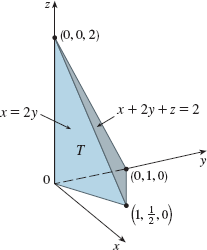
\includegraphics[width=4cm]{12_2_4} 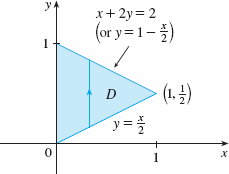
\includegraphics[width=6cm]{12_2_5}
  \end{center}

  Here we can see that the plane region $ D $ is bounded by the functions $ y=1-\frac{x}{2} ~\&~ y=\frac{x}{2} $. $ 1-\frac{x}{2} $ is obtained from $ x+2y=2 $ when $ z=0 $. However a simpler way to derive these bounds is to plot the equations $ x=2y $ and connect a line from the $ x ~\&~ y $ intercepts. The slope of the line gives us $ y=1-\frac{x}{2} $ and we set that equal to $ y=1-\frac{x}{2} $. 

  By then solving for where those two lines intersect, we will have drawn the plane region $ D $.

  The upper and lower bounds are $ y=1-\frac{x}{2} ~\&~ y=\frac{x}{2} $ respectively. The region also starts from $ x=0 $ and ends at $ x=1 $. Giving the region
  \[
    D= \{ (x,y) | 0 \le x \le 1, \frac{x}{2} \le y \le 1 - \frac{x}{2} \}
  \]

  Therefore
  \[
    \begin{gathered}
    V = \iint_D 2-x-2y~dA = \int^{1}_{0} \int^{1-\frac{x}{2}}_{\frac{x}{2}} 2-x-2y ~ dydx\\
    \int^{1}_{0} \text{\huge{[}} \int^{1-\frac{x}{2}}_{\frac{x}{2}} 2-x-2y ~ dy \text{\huge{]}}~dx = \int^{1}_{0} \text{\huge{[}} 2y-xy-y^{2} \text{\huge{]}}^{y=1-\frac{x}{2}}_{y=\frac{x}{2}}~dx\\
    \int^{1}_{0} \text{\huge{[}} 2-x-x(1-\frac{x}{2}) - (1-\frac{x}{2})^{2} - x + \frac{x^{2}}{2} + \frac{x^{2}}{4}\text{\huge{]}}~dx\\
    \int^{1}_{0} x^{2}-2x+1~dx = \frac{x^{3}}{3}-x^{2}+x \bigg|^{1}_0= \boxed{\frac{1}{3}}
    \end{gathered}
  \]
 
  \textbf{Ex 5}\\
  Evaluate the iterated integral $ \int^{1}_{0} \int^{1}_{x} \sin(y^{2}) ~ dydx $.

  Notice that the inner integral $ \int \sin(y^{2})~dy $ is simply impossible in finite terms. So we must rewrite the integral into a simpler form. The first approach is to go backwards.
  \[
   \int^{1}_{0} \int^{1}_{x} \sin(y^{2}) ~ dydx \to \iint_D \sin(y^{2})~dA   
  \]

  Where the plane region is
  \[
    D = \{ (x,y) | 0 \le x, x \le y \le 1 \}
  \]
  Which can be rewritten as
  \[
    D = \{ (x,y) | 0 \le y \le 1, 0 \le x \le y \}
  \]

  Converting the integral like so
  \[
    \begin{gathered}
    \int^{1}_{0} \int^{1}_{x} \sin(y^{2}) ~ dydx \to \iint_D \sin(y^{2})~dA \to \int^{1}_{0} \int^{y}_{0} \sin(y^{2}) ~dxdy\\
    \int^{1}_{0} \text{\huge{[}} \int^{y}_{0} \sin(y^{2})~dx \text{\huge{]}} dy = \int^{1}_{0} \text{\huge{[}} x\sin(y^{2}) \text{\huge{]}}^{x=y}_{x=0}~dy\\
    \int^{1}_{0} y\sin{(y^{2})}~dy = -\frac{1}{2}\cos{(y^{2})} \bigg|^{1}_{0}\\
    \frac{1}{2}(1-\cos{1})=\boxed{\frac{1-\cos{1}}{2}} 
    \end{gathered}
  \]
 
  \textbf{Properties of Double Integrals}
  \[
    \iint_D [f(x,y)+g(x,y)]~dA = \iint_D f(x,y)~dA + \iint g(x,y)~dA
  \]
  \[
    \iint_D cf(x,y)~dA = c \iint f(x,y)~dA
  \]

  If $ f(x,y) \ge g(x,y) \forall (x,y) \in D $, then
  \[
    \iint_D f(x,y)~dA \ge \iint g(x,y)~dA
  \]

  If $ D=D_1 \cup D_2 $, where $ D_1 ~\&~ D_2 $ don't overlap except perhaps on their boundaries then
  \[
    \iint f(x,y)~dA = \iint_{D_1} f(x,y)~dA + \iint_{D_2} f(x,y)~dA
  \]

  \begin{center}
    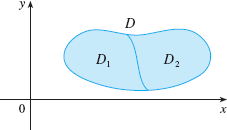
\includegraphics[width=6cm]{12_2_6}
  \end{center}

  The above integral can be used to evaluate double integrals over regions $ D $ that can be expressed as a union of regions of type I or type II. As shown below.
  \begin{center}
    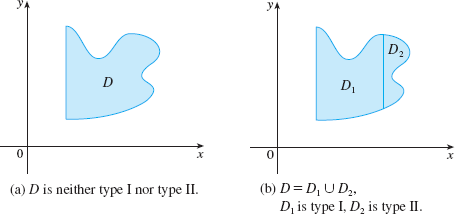
\includegraphics[width=10cm]{12_2_7}
  \end{center}

  If we integrate the constant function $ f(x,y)=1 $ over a region $ D $, we get the area of $ D $
  \[
    \iint_D 1~dA = A(D)
  \]
\end{document}
